\chapter[Simulado 3]{Simulado}

\vspace*{-.5cm}

\num{1} Durante a aula de matemática a professora colocou na lousa a
seguinte decomposição de um número:

\begin{mdframed}[linewidth=2pt,linecolor=salmao,backgroundcolor=salmao!20]
\centering
4 x 1.000 + 3 x 100 + 3 x 10 + 5 x 1
\end{mdframed}

Muito rapidamente, Artur levantou a mão e disse que sabia qual era o
número. Qual o número representado por essa decomposição?

\begin{multicols}{2}
\begin{escolha}
\item
  4.035
\item
  4.335
\item
  5.034
\item
  5.304
\end{escolha}
\end{multicols}


\num{2} Ricardo deseja escrever o maior número possível
utilizando os algarismos 1, 2, 4, 5 e 7, sem repeti-los nenhuma vez. Qual
o maior número que ele irá escrever?

\begin{escolha}
\item
  Setecentos e cinquenta mil e quatrocentos e vinte um
\item
  Setenta e cinco mil e quatrocentos e vinte um
\item
  Quarenta e cinco mil e duzentos e cinquenta e sete
\item
  Dezessete mil e quinhetos e quarenta e cinco
\end{escolha}

\num{3} A seguinte conta foi colocada no quadro durante uma aula de
matemática.

\begin{figure}[htpb!]
\centering
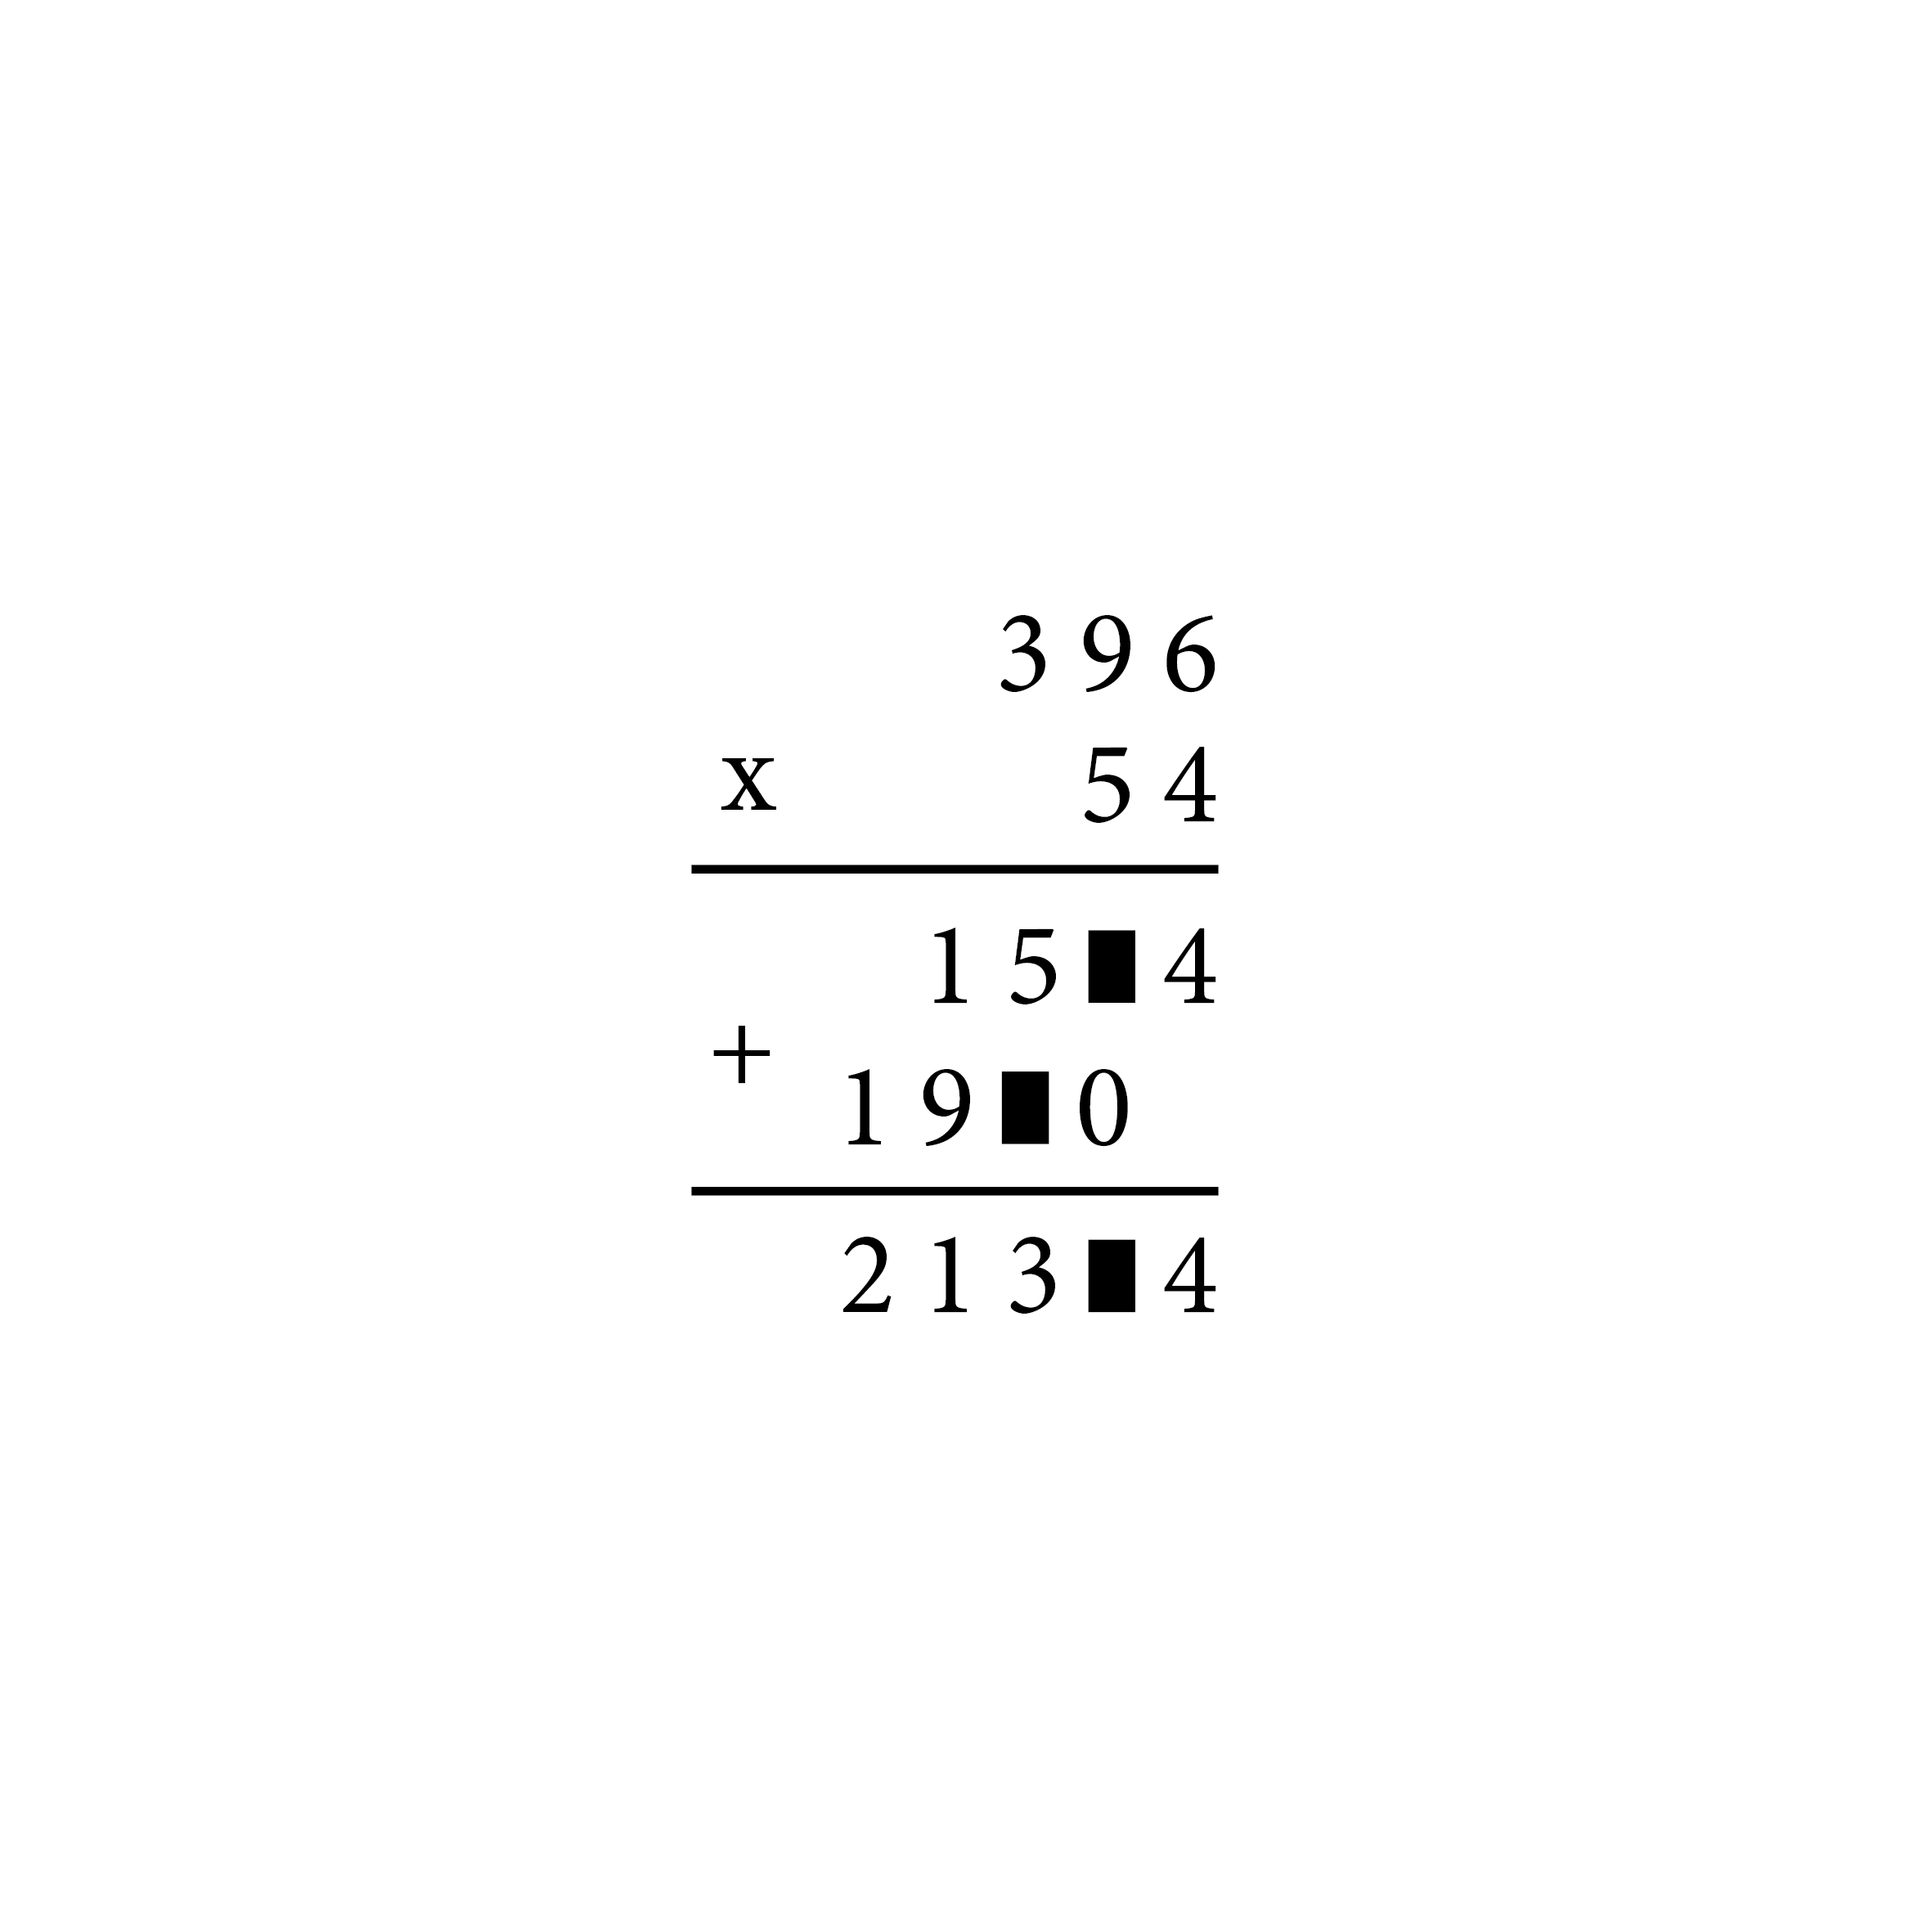
\includegraphics[width=.2\textwidth]{../ilustracoes/MAT5/SAEB_5ANO_MAT_figura121.png}
\end{figure}
%ATENÇÃO: essa imagem NÃO É CLARA. A impressão do leitor é que a primeira conta é 396 X 54. Mas essa não é a conta proposta. 396 X 4 = 1.584 (número da terceira linha) e 396 X 5 = 1.980 (número da quarta linha). A visualização proposta não é clara para qualquer leitor; será muito mais confusa para um aluno em formação. Fiz um gabarito simples, porque acredito que é preciso reformular essa imagem.   

Qual o número devemos colocar no lugar dos quadradinhos para que a conta
fique correta?

\begin{multicols}{2}
\begin{escolha}
\item
  2
\item
  6
\item
  7
\item
  8
\end{escolha}
\end{multicols}


\num{4} Alex estava observando a sequência numérica (3; 9; 27; 81; 243;
729). Pode-se dizer que para encontrarmos um elemento qualquer da
sequência devemos a um termo anterior:

%\begin{minipage}{.5\textwidth}
\begin{escolha}
\item
  Somar 6
\item
  Dividir por 3
\item
  Multiplicar por 3
\item
  Somar 9
\end{escolha}
%\end{minipage}


\num{5} O zoológico da cidade em que Fabiana mora abre às 9 horas da manhã
e fica aberto apenas 8 horas e meia por dia. Em que horário as atividades 
do zoológico são encerradas, sabendo-se que ele não fecha no horário do
almoço?

%\begin{minipage}{.5\textwidth}
\begin{escolha}
\item
  16h30
\item
  17h30
\item
  17h45
\item
  18h30
\end{escolha}
%\end{minipage}


\num{6} O programa preferido de Marquinhos na internet começa pontualmente
às 14h55 e termina exatamente às 15h34.
Qual a duração do programa favorito de Marquinhos?

%\begin{minipage}{.5\textwidth}
\begin{escolha}
\item
  39 minutos
\item
  45 minutos
\item
  50 minutos
\item
  1 hora e 20 minutos
\end{escolha}
%\end{minipage}


\num{7} Marina quer colocar um carpete de madeira no quarto de sua única
filha. Para isso representou o quarto da menina na malha quadriculada
abaixo, na qual a parte escura corresponde ao carpete de madeira que será
colocado.

\pagebreak
\begin{figure}[htpb!]
\centering
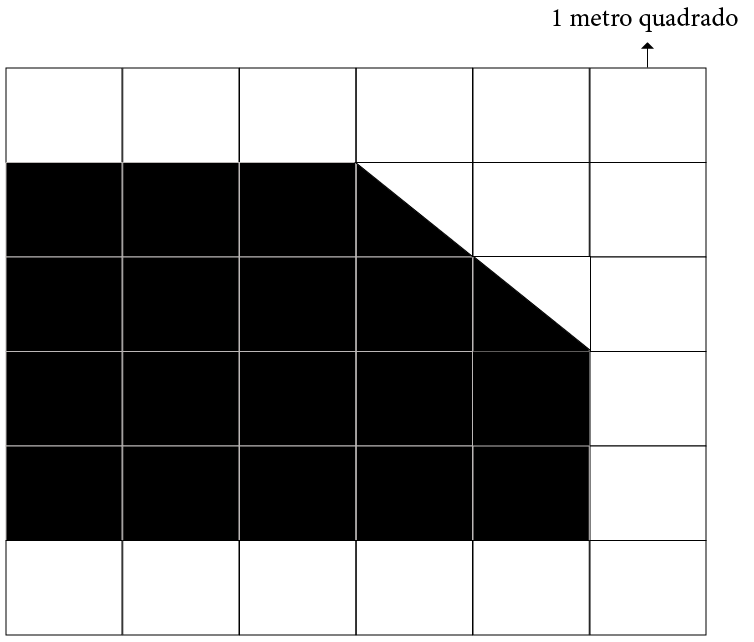
\includegraphics[width=.45\textwidth]{../ilustracoes/MAT5/SAEB_5ANO_MAT_figura122.png}
\end{figure}

Como cada quadradinho possui 1 metro quadrado de área, qual a área total
de carpete de madeira que ela terá que encomendar para colocar no quarto
da filha sem que falte nenhum pedaço e também não sobre material?\bigskip

\begin{multicols}{2}
\begin{escolha}
\item
  12 m²
\item
  17 m²
\item
  18 m²
\item
  20 m²
\end{escolha}
\end{multicols}


\num{8} Um cartão é retirado de forma aleatória de um conjunto de 50
cartões numerados de 1 a 50. Qual a probabilidade de que, no cartão
retirado, esteja escrito um número entre 20 e 40?

\begin{multicols}{2}
\begin{escolha}
\item
  15\%
\item
  38\%
\item
  56\%
\item
  74\%
\end{escolha}
\end{multicols}


\num{9} Um universítário recebeu seu extrato de notas:

\begin{longtable}[]{@{}ll@{}}
\toprule
Disciplinas & Notas\tabularnewline
\midrule
\endhead
II & 8,0\tabularnewline
III & 6,0\tabularnewline
IV & 5,0\tabularnewline
V & 7,5\tabularnewline
\bottomrule
\end{longtable}

Sabendo-se que a média para passar em cada disciplina é 6,00, a
disciplina em que ele foi reprovado é a:

\begin{multicols}{2}
\begin{escolha}
\item
  II
\item
  III
\item
  IV
\item
  V
\end{escolha}
\end{multicols}
\pagebreak

\num{10} Em uma seletiva para a fase final da prova de 100 metros livres
de natação, os 8 atletas que disputaram obtiveram os seguintes tempos:

\begin{center}
\begin{tabular}{l|c|c|c|c|c|c|c|c}
\hline
\textbf{Raia} & 1 & 2 & 3 & 4 & 5 & 6 & 7 & 8 \\ \hline
\textbf{\begin{tabular}[c]{@{}l@{}}Tempo\\ (segundo)\end{tabular}} & 20,90 & 20,90 & 20,50 & 20,80 & 20,60 & 20,60 & 20,90 & 20,96 \\ \hline
\end{tabular}
\end{center}

Sabendo-se que apenas os três mais velozes passam para a próxima fase,
podemos afirmar que os atletas classificados foram os das raias:

%\begin{minipage}{.5\textwidth}
\begin{escolha}
\item
  1, 3 e 8
\item
  3, 5 e 6
\item
  1, 7 e 8
\item
  5, 6 e 7
\end{escolha}
%\end{minipage}


\num{11} Um prêmio de R\$ 600,00 será dividido da seguinte forma
entre os três primeiros colocados:

\begin{itemize}
\item
  O primeiro receberá ½ do valor;
\item
  O segundo receberá 1/3 do prêmio;
\item
  O terceiro receberá o restante do prêmio.
\end{itemize}

Sendo assim, pode-se afirmar que o terceiro colocado receberá:

%Alterei o enunciado para a formulação acima ser usada de maneira integral. 

%%\begin{minipage}{.5\textwidth}
\begin{escolha}
\item
  R\$ 300,00
\item
  R\$ 200,00
\item
  R\$ 100,00
\item
  R\$ 50,00
\end{escolha}
%%\end{minipage}

\num{12} Durante um treino de futebol Camilo acertou 8 pênaltis dos 14
que bateu. Pode-se afirmar que a razão do número de pênaltis que ele
errou em relação ao total de pênaltis que ele bateu é:

%\begin{minipage}{.5\textwidth}
\begin{escolha}
\item
  4/7
\item
  3/7
\item
  3/4
\item
  4/3
\end{escolha}
%\end{minipage}


\num{13} Em uma cadeira reclinável o assento possui 3 opções de posições
diferentes e o encosto possui 5 opções de posições diferentes. Quantas
possibilidades de posições combinando uma posição para o assento e uma
posição para o encosto podemos formar:

\begin{multicols}{2}
\begin{escolha}
\item
  9
\item
  15
\item
  25
\item
  40
\end{escolha}
\end{multicols}


\num{14} Lucas, com o auxílio de seu professor está montando no
laboratório de robótica um super sistema de transmissão de dados.
Para isso, ele precisa de 7 metros de fio de cobre, cortados em 
pedaços menores de 0,14 metros de comprimento.

Ela já possui 8 pedaços no tamanho desejado. Quantos pedaços ainda
faltam para ele continuar a montar seu sistema?

\begin{multicols}{2}
\begin{escolha}
\item
  8
\item
  26
\item
  42
\item
  50
\end{escolha}
\end{multicols}



\num{15}
\begin{myquote}
  {[}\ldots{}{]} Existem muitos jeitos de brincar, mas o objetivo é sempre desfrutar o
  momento e a companhia dos amigos. Além disso, os jogos ajudam a
  desenvolver habilidades que serão importantes ao longo da vida.
  Brincar é também uma maneira de aprender!

Os índios possuem muitos jogos e brincadeiras. Alguns são bastante
conhecidos por vários povos indígenas, {[}\ldots{}{]} como a peteca e a perna
de pau. {[}\ldots{}{]}

\fonte{Mirim Povos Indígenas Brasil. Brincadeiras. Disponível em: \emph{
https://mirim.org/pt-br/como-vivem/brincadeiras}. Acesso em: 16 fev.
2023.}
\end{myquote}

\noindent{}Segundo o texto, algumas brincadeiras indígenas

\begin{escolha}
\item são parecidas com algumas brincadeiras tradicionais também não indígenas.

\item são realizadas exclusivamente pelos indígenas, sem influências ou compartilhamentos.

\item são padronizadas para os povos indígenas.

\item são praticadas de maneira individual.
\end{escolha}



\pagebreak
\num{16} Leia um trecho de notícia.
\begin{myquote}
  {[}\ldots{}{]} as crianças aprendem a respeitar o próximo, a ceder, a
  ganhar e a perder e constroem o senso de coletividade. Isso vai
  refletir no convívio com a família, na escola e, futuramente, até no
  trabalho.

\fonte{G1. Bem estar. Esporte coletivo promove o respeito ao próximo e o trabalho em equipe.
Disponível em: \emph{
https://g1.globo.com/bemestar/noticia/2016/08/esporte-coletivo-promove-o-respeito-ao-proximo-e-o-senso-de-coletividade.html}.
Acesso em: 16 fev. 2023.}
\end{myquote}

\noindent{}Depois da leitura, é possível perceber que o texto fala sobre

\begin{multicols}{2}
\begin{escolha}
\item os jogos pré-depsortivos.

\item os esportes competitivos.

\item as modalidades olímpicas.

\item as atividades escolares.
\end{escolha}
\end{multicols}
\enlargethispage{2\baselineskip}


\num{17} Observe a imagem.
  \begin{figure}[htpb!]

\includegraphics[width=\textwidth]{./imgs/img15.jpg}
\end{figure}
%Disponível em: https://br.freepik.com/fotos-gratis/dancarinas-nigerianas-de-tiro-medio\_16130625.htm\#\&position=34\&from\_view=collections. Acesso em: 16 fev. 2023.

\noindent{}Após a análise, pode-se perceber que é uma dança, pois

\begin{escolha}
\item as pessoas estão dançando ao ar livre.

\item as pessoas estão realizando uma pratica corporal coletiva.

\item as pessoas estão com vestimentas e pinturas corporais da dança.

\item as pessoas estão se movimentando no ritmo do batuque do instrumento
musical.
\end{escolha}



\pagebreak
\num{18} No estômago, o alimento é envolvido pelo suco gástrico.
Forma-se, assim, uma massa de bolo alimentar chamada quimo. Quando chega
ao intestino delgado, o quimo passa por ações de várias substâncias, que
aproveitam os nutrientes necessários, como o amido e as proteínas, e,
então, passa a ser chamado de quilo.

O texto descreve etapas do processo de

\begin{multicols}{2}
\begin{escolha}
\item digestão.

\item alimentação.

\item hidratação.

\item evacuação.
\end{escolha}
\end{multicols}



\num{19} A densidade nutricional de um alimento é uma classificação
que separa as calorias consumidas em cheias ou vazias. As calorias
cheias são as que fornecem quantidades de vitaminas, fibras, gorduras e
proteínas em equilíbrio, enquanto as vazias apresentam um número elevado
de açúcares e gorduras.

Alimentos com menor densidade nutricional apresentam calorias vazias,
pois

%\begin{minipage}{.5\textwidth}
\begin{escolha}
\item são alimentos com menor teor calórico.

\item são essenciais para qualquer dieta.

\item são uma fonte pobre de nutrientes.

\item são menos ofensivos ao organismo.
\end{escolha}
%\end{minipage}


\num{20} Ao estudar as fases da lua, um pesquisador observou o céu
todas as noites, a fim de anotar informações sobre a visibilidade do
satélite natural da Terra. Ele registrou as anotações numa tabela:

\begin{longtable}[]{@{}ll@{}}
\toprule
\textbf{Semana} & \textbf{Fase da lua}\tabularnewline
1 & Minguante\tabularnewline
2 & Nova\tabularnewline
3 & Crescente\tabularnewline
4 & Cheia\tabularnewline
\bottomrule
\end{longtable}

Com base nessas informações, observou que se tratava de um ciclo lunar
sinódico, no qual cada fase dura entre 7 e 8 dias.

No meio da semana 5, qual será a fase da lua?

%\begin{minipage}{.5\textwidth}
\begin{escolha}
\item Cheia.

\item Nova.

\item Crescente.

\item Minguante.
\end{escolha}
%\end{minipage}


\pagebreak